\subsection{ID regression}
The parameters within the two models have been identified with Inverse dynamics (ID) regression on a set of manoeuvring model tests with the WPCC. 

\label{sec:result_ID_regression}
\autoref{fig:ID_regression_ID_N}
%\begin{figure}[h!]
%    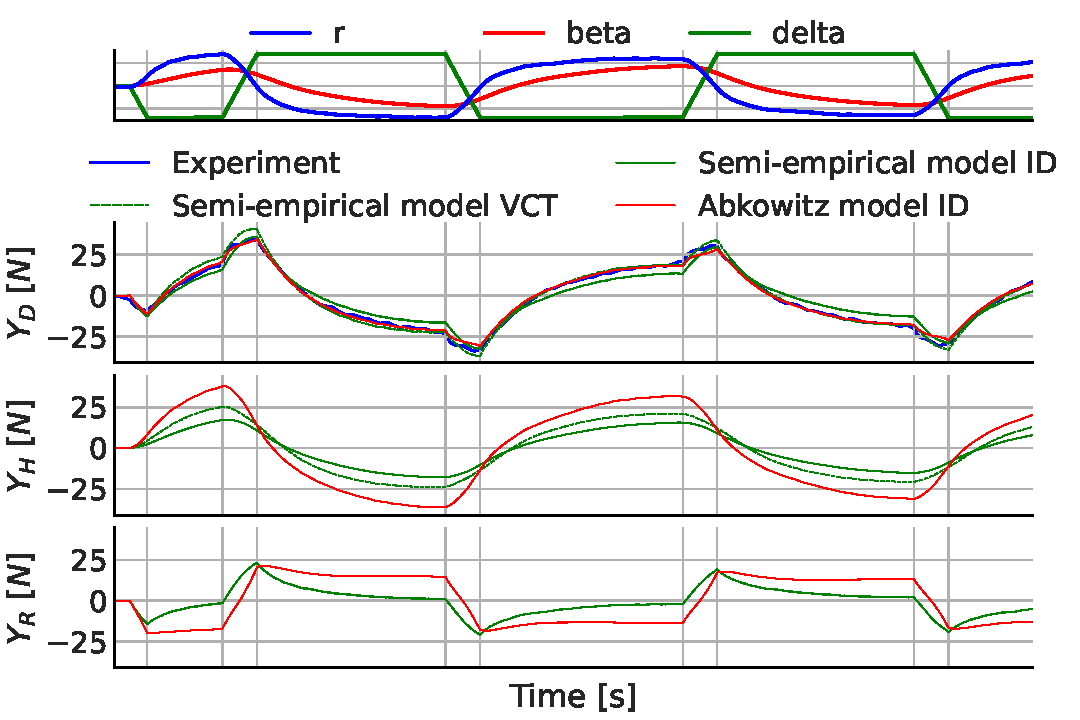
\includegraphics[width=\textwidth]{figures/result_ID_regression.ID_regression_ID_Y.pdf}
%    \caption{}
%    \label{fig:ID_regression_ID_Y}
%\end{figure}
\begin{figure}[h!]
    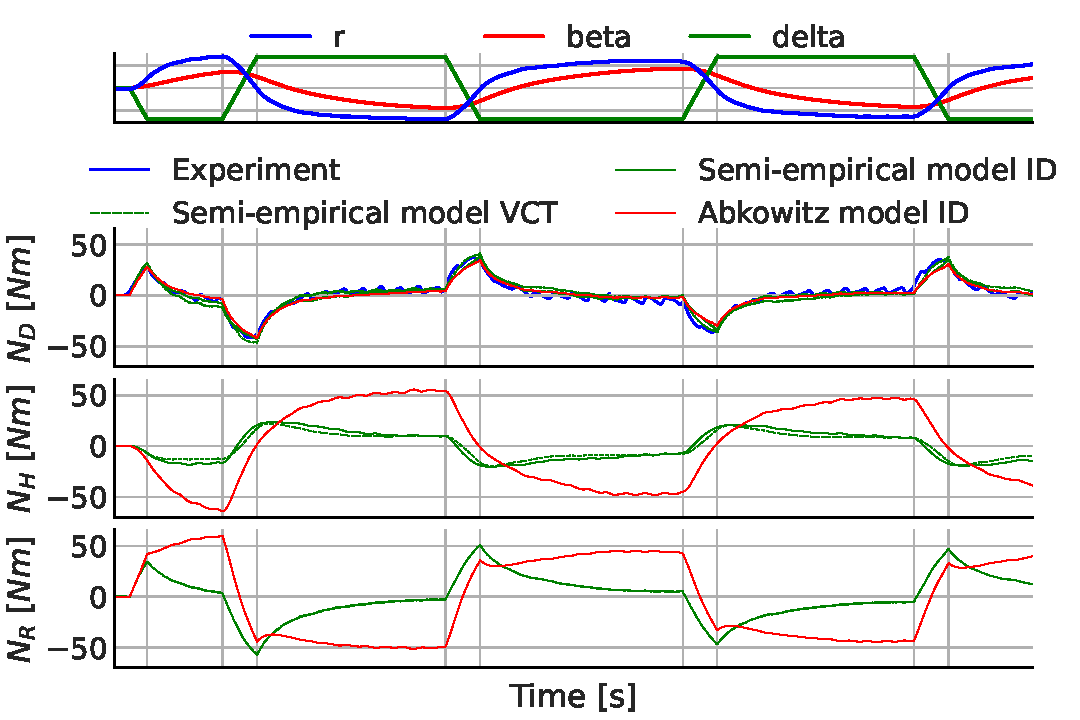
\includegraphics[width=\textwidth]{figures/result_ID_regression.ID_regression_ID_N.pdf}
    \caption{Comparison of the total yawing moment acting on the ship: predicted with the Semi-empirical VCT model, predicted with the Semi-empirical ID model, predicted with the Abkowitz ID model, and the corresponding values from a zigzag20/20 test estimated with inverse dynamics.}
    \label{fig:ID_regression_ID_N}
\end{figure}
